\documentclass{article}
\usepackage{graphicx} % Required for inserting images
%Welcome :)

\documentclass{article}

% Basic document formatting
\usepackage[utf8]{inputenc}     % Input encoding
\usepackage[T1]{fontenc}        % Font encoding
\usepackage{lmodern}            % Modern LaTeX fonts
\usepackage{geometry}           % Set page margins
\geometry{a4paper, total={170mm,257mm}, left=20mm, top=20mm} 
\usepackage{float}              % Handling of floating elements
\usepackage{fancyhdr}           % Fancy headers
\usepackage{lastpage}           % use \pageref{LastPage} to make page x of y footers
\setlength{\parindent}{0pt}     % No \noindent

% Figures
\usepackage{graphicx}           % For including images
\usepackage{caption}            % Using the caption package
\usepackage{wrapfig}            % For including Wrap Figures
\usepackage{subcaption}         % For subfigures within a figure environment
\usepackage{pgfplots}           % Drawing plots
\usepackage{pgf-pie}            % For creating pie charts
\captionsetup[figure]{labelfont=bf}
\captionsetup[table]{labelfont=bf}
\usepackage{asymptote}          % Zum Zeichnen verschiedener Plots 
\usepackage{pdfpages}           % Zum Einfügen ganzer PDFs

% Colorboxes
\usepackage[skins]{tcolorbox}   % Color Boxes

% Tables and long tables
\usepackage{tabularx}           % Advanced table features
\usepackage{longtable}          % For tables that span multiple pages
\usepackage{multirow}           % Allows for multirow cells in tables
\usepackage{booktabs}           % For professional-quality tables

% Math packages
\usepackage{amsmath}            % Enhanced mathematical formatting
\usepackage{amssymb}            % Extended symbol collection
\usepackage{amsfonts}           % Mathematical fonts
\usepackage[version=4]{mhchem}  % Chemische Formeln
\usepackage{mathtools}          % Mathematical tools to supplement amsmath
\numberwithin{equation}{section} % Numbers Equations with chapters
\usepackage{siunitx}            % Makes SI-Units

% Code display
\usepackage{listings}           % For displaying code
\usepackage{xcolor}             % For coloring code
\lstdefinestyle{mystyle}{
    backgroundcolor=\color{backcolour},   
    commentstyle=\color{codegreen},
    keywordstyle=\color{ao},
    numberstyle=\tiny\color{codegray},
    basicstyle=\ttfamily\footnotesize,
    breakatwhitespace=false,         
    breaklines=true,                 
    captionpos=b,                    
    keepspaces=true,                 
    numbers=left,                    
    numbersep=5pt,                  
    showspaces=false,                
    showstringspaces=false,
    showtabs=false,                  
    tabsize=2
}
\lstset{style=mystyle}

% Custom Colours
\definecolor{LightCyan}{rgb}{0.88,1,1}
\definecolor{dkgreen}{rgb}{0,0.6,0}
\definecolor{gray}{rgb}{0.5,0.5,0.5}
\definecolor{mauve}{rgb}{0.58,0,0.82}
\definecolor{codegreen}{rgb}{0,0.6,0}
\definecolor{codegray}{rgb}{0.5,0.5,0.5}
\definecolor{ao}{rgb}{0.0, 0.0, 1.0}
\definecolor{backcolour}{rgb}{0.95,0.95,0.92}

% Referencing
\usepackage[style=numeric, backend=biber, sorting=none]{biblatex} % Imports biblatex package
\addbibresource{MAIN.bib} %Import the bibliography file
\DeclareFieldFormat{labelnumberwidth}{\mkbibbrackets{#1}} %ensure that the label numbers in the bibliography are enclosed in brackets.
\usepackage{xurl}

% Hyperlinks in the document
\usepackage{hyperref}           % For adding hyperlinks


\begin{document}

\vspace{-4cm}

\includegraphics[width=0.25\linewidth]{Graphics/VCS-Logo.png}

\vspace{-1.5cm}
\begin{flushright}
\parbox[r]{4cm}{Zurich, \today}
\end{flushright}

\vspace{1.5cm} %nice danke
\begin{center}
\textbf{\LARGE{Proposal and Ideas of the VCS regarding PAKETH}} \\
\vspace{0.5cm}
\Large
VCS - Association of Students in Chemistry, Biochemistry – Chemical Biology, 
Chemical Engineering, and Interdisciplinary Natural Sciences
\end{center}

\section{Exam preparation time}
The VCS strongly favours \textbf{4 weeks} preparation time.

\section{Deregistration Deadline}
We believe that allowing a late exam deregistration grants our students flexibility. Deciding at the start of the semester which exams to take months later is a challenge. Many students need more than three weeks to assess whether to take all exams during the exam session. It has been especially noted in the third year of Chemical Engineering that many students postpone one of the two blocks from the autumn semester. \\

We see a significant advantage in delaying the deregistration from a course (and its exam) as much as possible, as it encourages students to enroll in challenging subjects. It is conceivable that fewer students would dare to do so if the option to withdraw from exams were removed.

\section{Retake Phase}
We agree with the proposal to offer retake exams before regular exams. It allows students to prepare for retakes first.

\section{Orientation Semester}
We consider the orientation semester as very important for students. The orientation semester is intended for students who have failed an exam block twice and are therefore excluded from their field of study. The orientation semester allows students to continue studying for one semester after failing and to take courses outside their previous field. This serves as orientation and offers a chance to prevent students from being directly excluded from the university context or having to quickly decide where to change to.\\

Given that exam results are only published a few days before the start of the new semester, we find it difficult to expect a person to decide so quickly on a new field of study/not continuing to study at ETH.\\

It is important to us that the orientation semester remains an option, at least for students who are excluded from their program after the second or third year, as they are particularly affected.

\newpage
\section{First-Year Schedule Proposal}
Our predecessors initiated an effort to develop a revised schedule proposal. We have discussed it with students and see several advantages in dividing first year students into two groups. Lectures are offered in the morning, and lab times are split across Monday, Tuesday, Wednesday, and Thursday afternoons. This allows more students to participate in practicals during the semester, which is desirable during PAKETH times.

\begin{center}
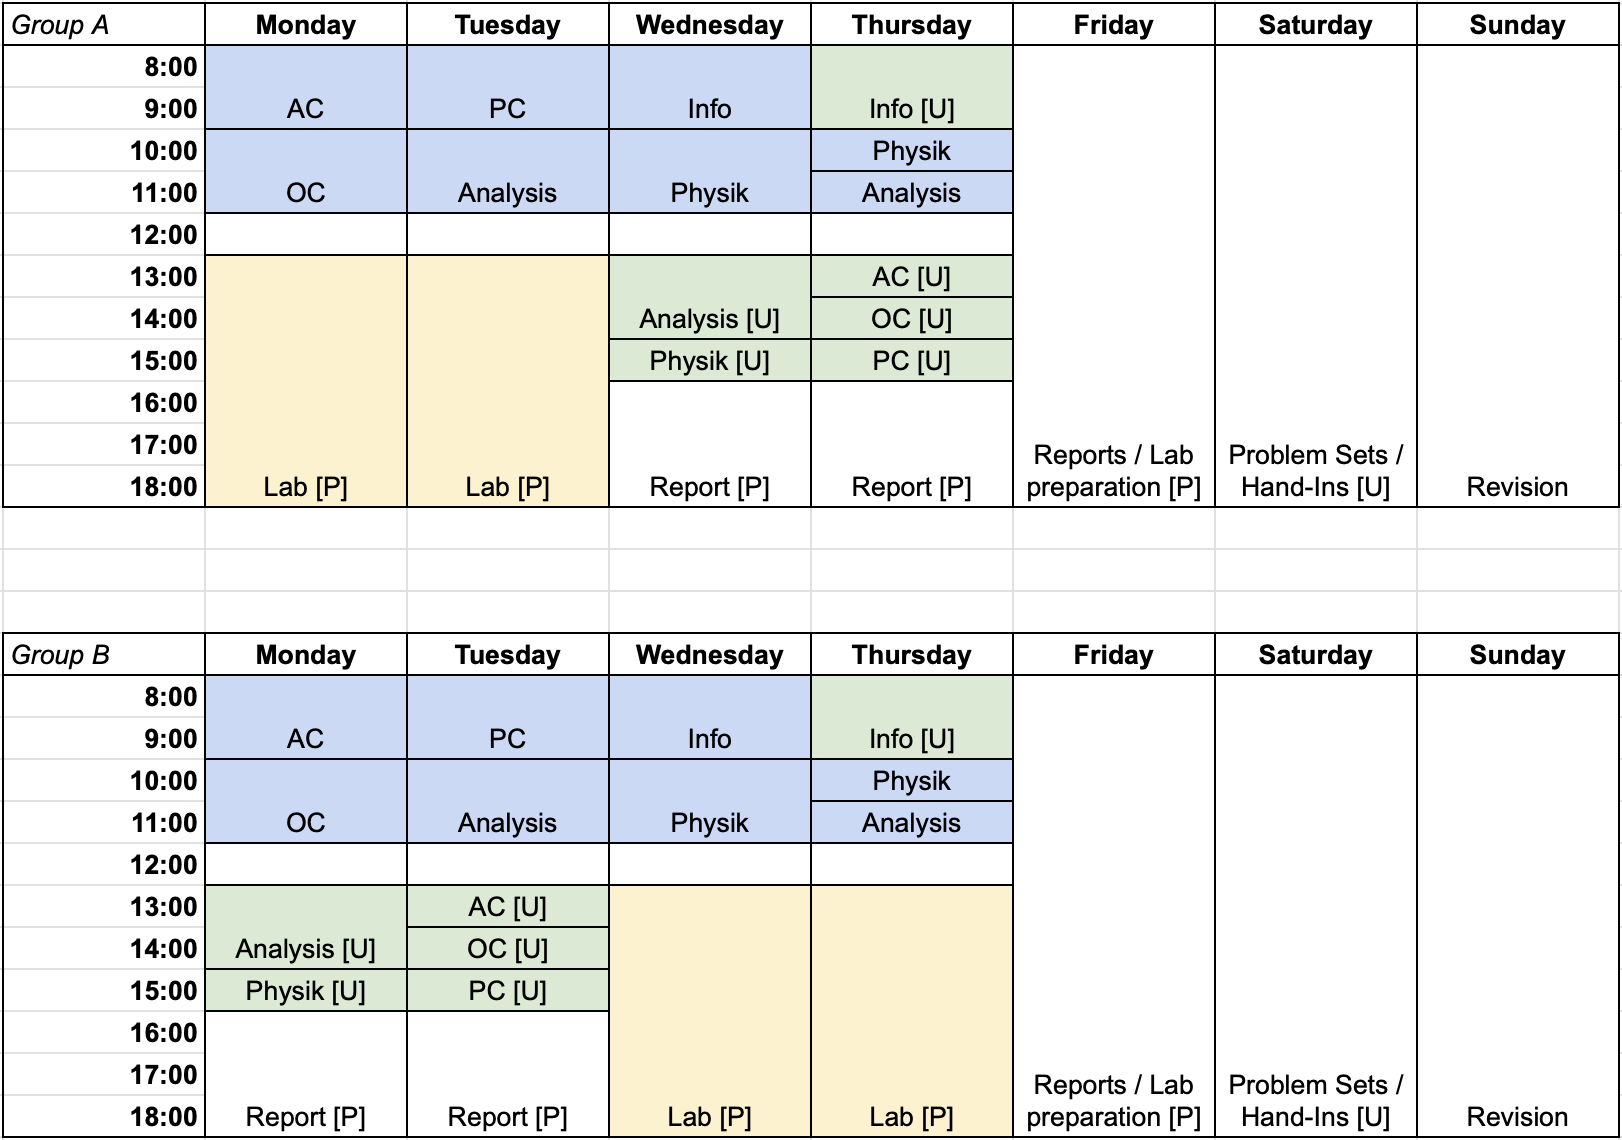
\includegraphics[width=0.9\linewidth]{Graphics/Screenshot 2024-11-08 at 07.54.10.png}
\end{center}

\end{document}
